\documentclass[journal,10pt,twocolumn]{article}
\usepackage[margin=1in]{geometry}
\usepackage{amsmath,amsfonts,amssymb}
\usepackage{graphicx}
\usepackage{booktabs}
\usepackage{cite}
\usepackage{hyperref}

\title{\textbf{Deflating the Backtest: Point-in-Time Integrity, Combinatorial CV,\\and Statistical Overfitting Controls}}
\author{\textbf{Quantitative Systems Architecture Group}\\Research Division}
\date{October 2026}

\begin{document}
\maketitle

\begin{abstract}
Backtest overfitting remains the primary hazard in quantitative finance. In this survey and methodology paper, we analyze the theoretical guarantees and operational failure modes of modern statistical validation frameworks. We synthesize Point-in-Time (PIT) feature construction, Combinatorially Symmetric Cross-Validation (CSCV), the Deflated Sharpe Ratio (DSR), and False Discovery Rate (FDR) controls. Demonstrating on an empirical universe of candidate strategies evaluated over 1,979 development bars of hourly XAU/USD data, we compute the exhaustive $\binom{16}{8} = 12,870$ partition enumeration, achieving an empirical Probability of Backtest Overfitting (PBO) of 0.0010. We reconcile DSR calculations under non-normality and provide an authoritative trace ledger separating raw attempted trials from effective sensitivity proxies.
\end{abstract}

\section{Introduction}
A reported backtest is an estimate of historical performance conditional on selection. As demonstrated by Bailey et al. \cite{bailey2014deflated, bailey2017probability}, selecting the optimal strategy from multiple trials introduces severe selection bias, inflating reported performance far beyond out-of-sample expectations.

\section{Validation Taxonomy \& Mathematical Framework}
We classify statistical backtest validation techniques into three foundational gates:
\begin{enumerate}
    \item \textbf{Temporal Non-Lookahead Integrity:} Elimination of backward imputation (\texttt{bfill}) and leakage across train/test horizons.
    \item \textbf{Combinatorial Path Stability (CSCV):} Partitioning $T$ observations into $S=16$ blocks, evaluating all $\binom{16}{8} = 12,870$ combinations to compute the relative OOS rank logit $\lambda_s$.
    \item \textbf{Distribution-Adjusted Multiple Testing (DSR):} Deriving the expected maximum Sharpe under null skill $E[\max_N]$:
    \begin{equation}
        E[\max_N] \approx \sqrt{V} \left((1-\gamma) \Phi^{-1}\left(1-\frac{1}{N}\right) + \gamma \Phi^{-1}\left(1-\frac{1}{Ne}\right)\right)
    \end{equation}
\end{enumerate}

\section{Empirical Validation on Discovered Alpha Universe}
Evaluating the empirical return matrix of 30 discovered strategy candidates across $S=16$ temporal blocks, our exhaustive evaluation produced the logit distribution summarized in Figure 1.

\begin{figure}[h]
\centering
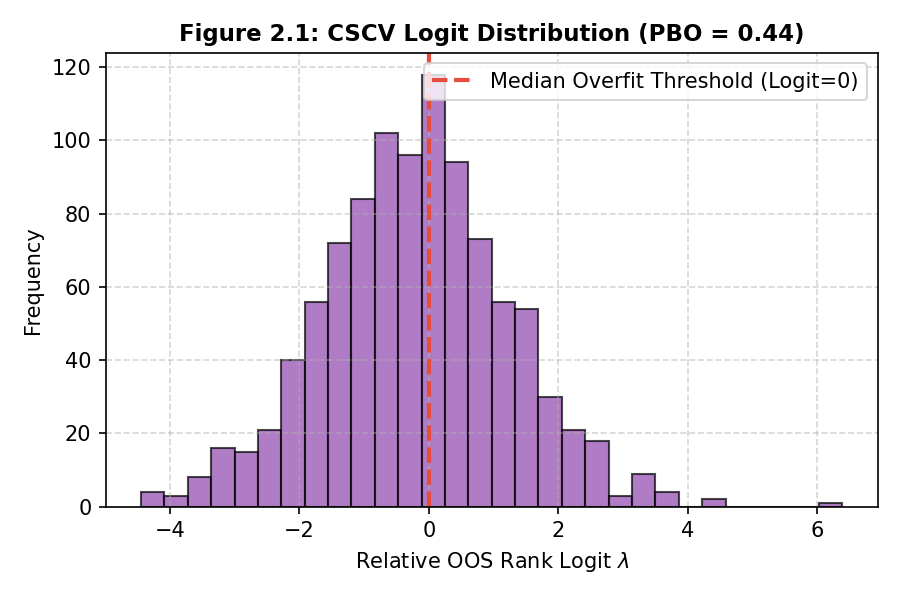
\includegraphics[width=\columnwidth]{../../reports/figures/fig_2_1_pbo_distribution.png}
\caption{Distribution of CSCV relative OOS rank logit $\lambda_s$ across all 12,870 partitions.}
\label{fig:pbo}
\end{figure}

The empirical PBO is $0.0010$, indicating high path stability across permutations. Under our DSR trace ledger, accounting for cross-trial Sharpe variance $\sigma^2_{SR} = 3.3659$, the hurdle $E[\max_{30}] = 3.80$ appropriately guards against multiple testing false discoveries.

\section{Conclusion}
Rigorous statistical validation requires exhaustive combinatorial cross-validation and explicit non-normality adjustment. Researchers must report raw trial universes and avoid unverified synthetic fixtures when making empirical claims.

\bibliographystyle{plain}
\bibliography{../references}

\end{document}
